% https://github.com/MCG-NKU/NSFC-LaTex
% https://www.overleaf.com/read/jydxqkkkskzp
% by Ming-Ming Cheng https://mmcheng.net
% 关于VsCode LaTeX的配置 https://www.cnblogs.com/ourweiguan/p/11785660.html

\documentclass[12pt]{article}


\usepackage[UTF8]{ctex}
\usepackage{nsfc}


%\usepackage{fontspec}
%\usepackage{xcolor}
%\defaultfontfeatures{Ligatures=TeX}




\newcommand{\lyc}[1]{\textcolor[rgb]{0,0.6,0}{LYC: #1}}
\newcommand{\todo}[1]{{\textcolor{red}{\bf [#1]}}}
\newcommand{\myPara}[1]{\paragraph{#1:}}

\graphicspath{{figures/}}


\begin{document}



%%%%%%%%% TITLE

\title{科研陈述}

\maketitle


\begin{center} {李元春} \end{center}



% 本人研究兴趣为软件工程、移动计算和人工智能的交叉领域,尤其关注移动端和云端大数据平台及人工智能软件中的隐私、安全、可靠性等问题,在相关领域顶级会议(如ICSE,FSE,ISSTA,UbiComp,MobiCom,SIGIR等)上发表论文二十余篇,其中包括CCF-A类会议第一作者长文9篇、短文或工具论文2篇。本人主导的工作获得了CCF A类会议UbiComp的最佳论文提名奖,以及领域知名会议IS-EUD的最佳论文奖,相关工具在开源软件平台上被广泛应用。
1991年,Mark Weiser 提出了普适计算(Ubiquitous Computing)的构想,主张将计算嵌入到环境或日常工具中去,使人能随时随地自然地使用各种计算服务。如今,这一构想已成为现实,以智能手机、智能汽车、机器人等为代表的移动和物联网终端设备迅速发展,在我们日常生活中扮演着越来越重要的角色。同时,随着近年来人工智能技术的飞速进步,将人工智能与普适计算技术结合起来已成为大势所趋。一方面,终端设备上丰富的数据可以为机器学习模型提供养料,另一方面,优秀的模型又可以极大地拓宽和改善终端设备提供的服务。我们正加速进入智能物联(AIoT)时代。

软件是AIoT的核心,在AIoT生态中,包括云端、边缘端、终端设备上都运行着各式各样的系统和软件,提供着丰富的服务。AIoT软件的可靠性(Reliability)是其长远发展中的关键主题之一,其包含两方面的含义,一方面是AIoT系统是否能够保障生态系统中每一方的权利和利益,如个人隐私、知识产权等。另一方面是AIoT提供的服务是否足够健壮和可信,避免产生故障或遭受攻击。
随着用户意识的觉醒、商业利益的考虑、以及各地政府政策的出台,AIoT的可靠性在产业中的重要性越来越凸显。

我主要面向AIoT的可靠性展开研究,大部分工作由真实问题驱动,从软件分析和系统设计的角度寻找问题的解决方案。如图~\ref{fig:overview}所示,我的工作面向AIoT生态中流通的三个关键对象,即数据、应用程序和机器学习模型,分别研究数据的隐私与合规、应用的分析与测试、以及模型的健壮性与安全性。


\begin{figure}
    \centering
    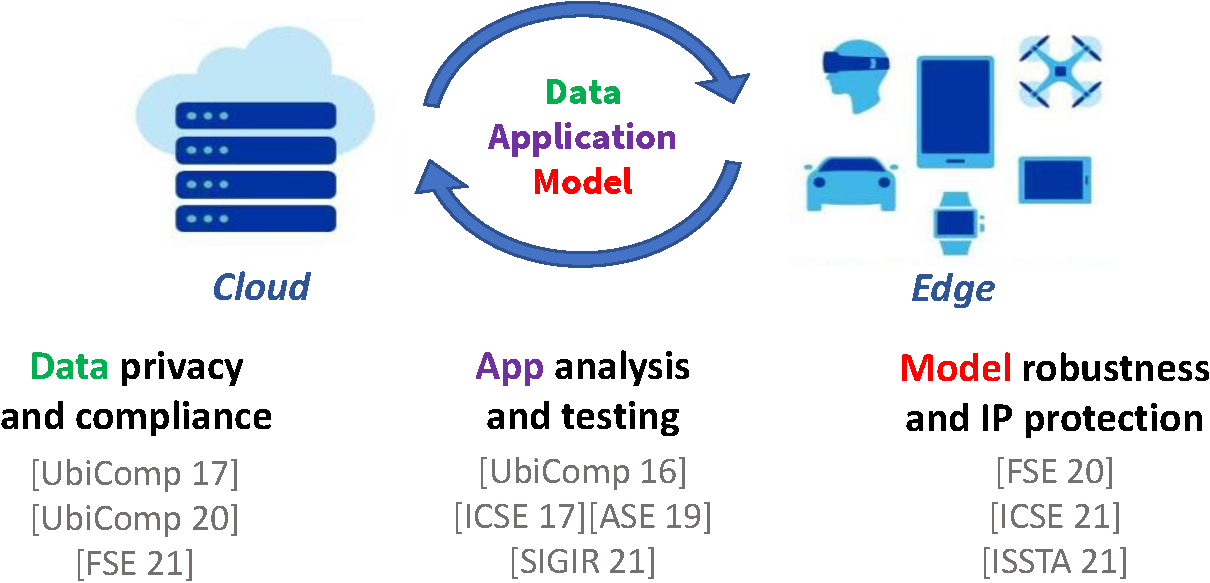
\includegraphics[width=5in]{figures/research_overview.pdf}
    \caption{研究工作概览}
    \label{fig:overview}
\end{figure}

\section{代表性工作}

\subsection{云-端协同数据处理及隐私保护框架}

数据是人工智能技术的重要基石,能否获得合适的数据是人工智能服务成功的关键。如今无处不在的移动和IoT设备是一个非常重要的数据来源,而如何在处理这些数据时尊重用户的隐私是一个必须解决的问题。
我的研究工作是从数据处理框架设计的角度出发,尝试创造一个云端统一、简单易用、保护隐私的个人数据处理框架。具有代表性的是 PrivacyStreams~\cite{li2017privacystreams} 和 TaintStream~\cite{yang2021taintstream} 系列工作。

我们观察到,云端和终端的数据处理方式是截然不同的。在云端和数据中心中,数据处理往往采用成熟统一的的流式处理框架(如 Spark),而在移动系统中,个人数据的组织形式十分异构,处理方式非常碎片化。例如在Android系统中,访问位置、读取通讯录、录音等分别有各自的接口,其数据处理操作也很分散和任意,难以进行隐私审查。
因此,我们提出了一个全新的移动端流式数据处理框架 PrivacyStreams,通过基于大量实证分析的编程接口设计,使移动应用开发者可以用与Spark类似的方式方便地访问和处理移动端各类个人和传感数据。同时,我们结合静态代码分析,可以对程序中使用的隐私数据处理流程和粒度进行分析。基于由真实开发者参与的用户实验,我们证明了 PrivacyStreams 可以在一些常见任务上将开发效率提升一倍,并使得开发的程序更加隐私透明。

PrivacyStreams 将云端和终端的数据处理方式统一成了基于流的形式。更进一步,我们考虑如何在这种流式数据平台中进行自动的隐私合规约束。这个问题也是目前大部分公司很关心的问题,由于GDPR等规定的施行,很多公司需要耗费大量人工检查各种隐私合规问题,比如数据留存,访问控制,用户退出等等。污点追踪(Taint Tracking)是一个学术界常用的隐私保护技术,通常通过修改系统监控敏感数据流动,但在这种大数据平台实现起来非常复杂。于是我们提出了一个新的框架 TaintStream,通过动态代码翻译的方法实现了轻量级、细粒度的污点追踪,基本的思路是让原始的代码在运行时自动转变成具有相同功能,但会同时传播污点标签的代码。基于这套系统,我们可以高精度、低代价地自动对数据进行各种隐私管理,从而大大降低人工进行隐私合规性检查的成本。

这一系列工作发表在普适计算和软件工程的顶级会议上,在开源社区取得了一定知名度(200+ stars)\cite{privacystreams:code},并受到了国内外媒体的报导。

% 数据的获取和处理是机器学习的关键步骤,尤其是移动端的数据具有很大的利用价值。而同时,由于移动端数据的高度敏感性,以及如今世界各国严格的隐私保护要求(如GDPR等),保护移动用户的隐私也尤为关键。本工作提出一个移动端隐私数据编程框架,在向开发者提供简单易用的流式编程接口的同时,减少代码数据流的碎片化,并进一步通过静态分析获取数据操作的敏感程度。该成果\cite{li2017privacystreams}发表在普适计算领域CCF-A类会议UbiComp 2017中,其对应工具在GitHub获得200多个星标\cite{privacystreams:code},并受多家媒体报道。

\subsection{基于交互界面的应用程序分析与测试}

应用程序是移动和IoT终端软件的主要表现形式,如今各平台上的应用数量已经以数百万记,如何自动测试和分析这些应用程序是一个重要的研究问题。

我的研究工作以软件的图形交互界面(UI)为切入点,对应用程序的功能和隐私特性进行分析。以UI为切入点有两方面优势:其一,UI是一种通用的信息形式,几乎所有应用程序都具有UI,且UI都遵循相似的设计模式,这对自动分析提供了便利。其二,应用程序的运行都是由UI交互驱动的,因此可以分析UI与代码的关联从而更细粒度地理解应用的功能。

我首先在应用程序自动测试输入生成方面做了一些工作。自动测试输入生成是软件测试里面的核心问题之一,直接决定了软件缺陷的发现效果。我们设计了一套轻量级的自动测试方法,可以在不插桩应用和系统的情况下,根据应用运行时的界面和状态信息决定测试输入。同时,我们通过对大量应用交互序列进行机器学习,自动学习到应用程序的交互模式,基于这些交互模式指导测试输入工具更加高效地测试应用。
更进一步,基于动态测试时获取的应用代码执行信息,可以结合代码静态分析方法,提取出应用界面与程序代码间的对应关系,例如每个交互动作会对应什么样的隐私数据访问等。这样的应用行为与界面的对应关系可以用来理解和自动判别软件中的隐私数据访问行为是否合理。

该工作的相关成果\cite{li2016peruim,li2017droidbot,liu2020pmc,li2019humanoid} 发表在领域顶级会议,并在 UbiComp 会议中并获得最佳论文提名奖,其相关联工具 DroidBot 在开源代码托管平台GitHub获得500多个星标\cite{droidbot:code},为领域内熟知。
 

\subsection{基于程序分析的模型安全分析与保障}

神经网络模型被认为是新一代的软件形态(Software 2.0),并越来越多地被应用在边缘端的安全攸关的场景中,如人脸验证、自动驾驶、安防监控等。因此其健壮性和安全性非常重要,但这也对软件分析与验证技术提出了新的要求。

我在这个方向的工作主要研究传统的软件分析方法能否以及如何应用到神经网络模型的分析与保护上。
例如,程序切片技术是传统程序分析、调试、测试的重要方法之一,旨在从程序代码中提取出与特定关注对象(如变量、API等)相关的子集(切片)。我的工作探索了在神经网络中实现程序切片技术的可行性和可能应用。我们提出一种基于正向和反向数据流分析的方法,给定一组输入和输出,可以提取出在模型决策过程中,对预测结果贡献关键作用的神经元子集。该切片技术可以用来分析和解释神经网络决策逻辑,例如可以通过切片模式的差异检测对抗样本、根据神经元的贡献大小对模型进行剪枝等等。
在另一个工作中,我们探讨了传统软件中的逆向工程技术能否用于神经网络模型的攻击,我们提出了一个直接在模型计算图上插入恶意旁路的攻击方法,可以在不需要训练的情况下,向目标模型中插入高效、轻量级的后门攻击。通过对两万多个真实移动应用的扫描分析,我们成功攻击了52个应用中的模型,其中包括下载量数千万的流行应用和安全攸关的支付、商业、儿童教育类应用。
我们还研究了将测试技术用于神经网络知识相似性的分析,通过生成有代表性的测试用例,可以根据模型对测试用例的反应判断模型之间是否有复用关系(如迁移学习的 teacher-student 关系),进而用来辅助保护模型的知识产权。
相关成果\cite{li2021deeppayload,zhang2020dynamic,li2021modeldiff}发表在软件工程领域顶级会议中。


\section{未来研究计划}

我计划继续沿着\textbf{AIoT软件可靠性}的方向进行研究,同时更加关注系统层面和方法论层面的创新。主要包括如下两方面的工作:


\textbf{面向软件2.0的程序开发、分析、验证方法}。
随着AI技术的进一步发展,传统程序与AI模型必将走向更深度的融合,软件的编程范式也将发生改变。未来运行在各个设备上的软件将不再是单纯的由传统的代码编译而成的可执行文件,而是代码和模型的有机结合,如何设计、分析及验证这类软件将是一个重要的研究问题,要求设计新的分析方法或对一系列传统软件技术进行方法层面的创新。我在之前的研究工作中积累了传统软件分析以及将传统程序分析方法用于神经网络分析的经验,在此基础上,我计划继续深入,基于产业界对AI软件可靠性的真实需求,探索更实用、更通用的新型软件设计和分析技术。

\textbf{面向AIoT的基础系统和框架}。
如今,IoT设备已经无处不在,这些设备在物理层面已经做到了高密度的互联(通过WiFi,蓝牙等),而在功能和语义层面还是相互孤立的。例如在智慧工厂或智能家居场景中,往往是有很多个IoT设备,每个设备分别独立地完成感知和计算任务,而多设备之间的联动、调度、以及知识的共享并没有系统层面的支持。即使是华为最近推出的主打万物互联的“鸿蒙”操作系统,也是为单个设备而设计。因此,如何为多AIoT设备形成的群体设计系统是一个重要的问题。这要求我们对系统进行更高级别的抽象,向下将IoT设备看作可使用和调度的资源,向上提供面向更具有语义的编程接口,以更简单和可靠的方式完成各种感知和计算任务。我在隐私数据框架设计方面积累了一定的系统经验,希望更进一步,为这种新的计算场景进行系统设计和研究。


% 如何理解自然界中的群体智能以及实现人工群体智能是我个人非常感兴趣的研究问题,移动设备丰富的传感能力和逐渐增强的计算能力为群体智能的发展提供了前所未有的机遇。受普适计算领域的众包、群智感知等概念的启发,我希望进一步研究如何让移动个体之间共享知识、共同学习,从而处理更大规模的感知和决策问题,例如如何让家庭和工厂中的智能设备自动协调合作、如何利用泛在的移动设备自动感知城市和环境的状态等等。这其中涉及到系统的搭建、大规模学习节点的性能、容错性,以及节点之间的隐私性等问题亟待解决。


{
\bibliographystyle{ieee_fullname}
\bibliography{lyc}
}


\end{document}
